	
% This template from http://www.vel.co.nz, originally from http://www.tedpavlic.com

\documentclass{article}
% Change "article" to "report" to get rid of page number on title page
\usepackage{amsmath,amsfonts,amsthm,amssymb, mathrsfs}
\usepackage{bigints}
\usepackage{setspace}
\usepackage{Tabbing}
\usepackage{fancyhdr}
\usepackage{lastpage}
\usepackage{textcomp}
\usepackage{extramarks}
\usepackage{chngpage}
\usepackage{soul,color}
\usepackage{graphicx,float,wrapfig}
\usepackage{cancel}
\usepackage{indentfirst}
\usepackage{mdframed}

% In case you need to adjust margins:
\topmargin=-0.45in      %
\evensidemargin=0in     %
\oddsidemargin=0in      %
\textwidth=6.5in        %
\textheight=9.0in       %
\headsep=0.25in         %

% Homework Specific Information
\newcommand{\hmwkTitle}{WS11}
\newcommand{\hmwkDueDate}{}
\newcommand{\hmwkClass}{Ay\ 190}
\newcommand{\hmwkAuthorName}{Cutter\ Coryell}

% Setup the header and footer
\pagestyle{fancy}                                                       %
\lhead{\hmwkAuthorName}                                                 %
\chead{\hmwkClass\ : \hmwkTitle}  %
\rhead{\hmwkDueDate}                                                     %
\renewcommand\headrulewidth{0.4pt}                                      %
\renewcommand\footrulewidth{0.4pt}                                      %

% This is used to trace down (pin point) problems
% in latexing a document:
%\tracingall

%%%%%%%%%%%%%%%%%%%%%%%%%%%%%%%%%%%%%%%%%%%%%%%%%%%%%%%%%%%%%
% Some tools
\newcommand{\enterProblemHeader}[1]{\nobreak\extramarks{#1}{#1 continued on next page\ldots}\nobreak%
                                    \nobreak\extramarks{#1 (continued)}{#1 continued on next page\ldots}\nobreak}%
\newcommand{\exitProblemHeader}[1]{\nobreak\extramarks{#1 (continued)}{#1 continued on next page\ldots}\nobreak%
                                   \nobreak\extramarks{#1}{}\nobreak}%

\newlength{\labelLength}
\newcommand{\labelAnswer}[2]
  {\settowidth{\labelLength}{#1}%
   \addtolength{\labelLength}{0.25in}%
   \changetext{}{-\labelLength}{}{}{}%
   \noindent\fbox{\begin{minipage}[c]{\columnwidth}#2\end{minipage}}%
   \marginpar{\fbox{#1}}%

   % We put the blank space above in order to make sure this
   % \marginpar gets correctly placed.
   \changetext{}{+\labelLength}{}{}{}}%

\setcounter{secnumdepth}{0}
\newcommand{\homeworkProblemName}{}%
\newcounter{homeworkProblemCounter}%
\newenvironment{homeworkProblem}[1][Problem \arabic{homeworkProblemCounter}]%
  {\stepcounter{homeworkProblemCounter}%
   \renewcommand{\homeworkProblemName}{#1}%
   \section{\homeworkProblemName}%
   \enterProblemHeader{\homeworkProblemName}}%
  {\exitProblemHeader{\homeworkProblemName}}%

\newcommand{\problemAnswer}[1]
  {\noindent\fbox{\begin{minipage}[c]{\columnwidth}#1\end{minipage}}}%

\newcommand{\problemLAnswer}[1]
  {\labelAnswer{\homeworkProblemName}{#1}}

\newcommand{\homeworkSectionName}{}%
\newlength{\homeworkSectionLabelLength}{}%
\newenvironment{homeworkSection}[1]%
  {% We put this space here to make sure we're not connected to the above.
   % Otherwise the changetext can do funny things to the other margin

   \renewcommand{\homeworkSectionName}{#1}%
   \settowidth{\homeworkSectionLabelLength}{\homeworkSectionName}%
   \addtolength{\homeworkSectionLabelLength}{0.25in}%
   \changetext{}{-\homeworkSectionLabelLength}{}{}{}%
   \subsection{\homeworkSectionName}%
   \enterProblemHeader{\homeworkProblemName\ [\homeworkSectionName]}}%
  {\enterProblemHeader{\homeworkProblemName}%

   % We put the blank space above in order to make sure this margin
   % change doesn't happen too soon (otherwise \sectionAnswer's can
   % get ugly about their \marginpar placement.
   \changetext{}{+\homeworkSectionLabelLength}{}{}{}}%

\newcommand{\sectionAnswer}[1]
  {% We put this space here to make sure we're disconnected from the previous
   % passage

   \noindent\fbox{\begin{minipage}[c]{\columnwidth}#1\end{minipage}}%
   \enterProblemHeader{\homeworkProblemName}\exitProblemHeader{\homeworkProblemName}%
   \marginpar{\fbox{\homeworkSectionName}}%

   % We put the blank space above in order to make sure this
   % \marginpar gets correctly placed.
   }%

\newenvironment{myindentpar}[1]%
 {\begin{list}{}%
         {\setlength{\leftmargin}{#1}}%
         \item[]%
 }
 {\end{list}}

%%%%%%%%%%%%%%%%%%%%%%%%%%%%%%%%%%%%%%%%%%%%%%%%%%%%%%%%%%%%%


%%%%%%%%%%%%%%%%%%%%%%%%%%%%%%%%%%%%%%%%%%%%%%%%%%%%%%%%%%%%%
% Make title
\title{\vspace{2in}\textmd{\textbf{\hmwkClass:\ \hmwkTitle}}\\\normalsize\vspace{0.1in}\small{Due\ on\ \hmwkDueDate}\\\vspace{0.1in}\large{\textit{\hmwkClassInstructor\ \hmwkClassTime}}\vspace{3in}}
\date{}
\author{\textbf{\hmwkAuthorName}}
%%%%%%%%%%%%%%%%%%%%%%%%%%%%%%%%%%%%%%%%%%%%%%%%%%%%%%%%%%%%%

%%%% MY COMMANDS %%%%%%%%%%%%%%%%%%%%%

\newcommand{\deri}[2]{\frac{\mathrm{d} #1}{\mathrm{d} #2}}
\newcommand{\pderi}[2]{\frac{\partial #1}{\partial #2}}
\newcommand{\inte}[4]{\int_{#1}^{#2} \! #3 \, \mathrm{d} #4}
\newcommand{\ointe}[4]{\oint_{#1}^{#2} \! #3 \, \mathrm{d} #4}
\newcommand{\del}{\nabla}
\newcommand{\D}{\mathrm{d}}
\newcommand{\ee}[1]{\times 10^{#1}}
\newcommand{\fpe}{\frac{1}{4 \pi \epsilon_0}}
\newcommand{\bra}[1]{\left< #1 \right|}
\newcommand{\ket}[1]{\left| #1 \right>}
\newcommand{\cket}[1]{\left. #1 \right>}


% Distance units
\newcommand{\m}[0]{\text{\ m}}
\newcommand{\cm}[0]{\text{\ cm}}
\newcommand{\km}[0]{\text{\ km}}
\newcommand{\pc}[0]{\text{\ pc}}
\newcommand{\kpc}[0]{\text{\ kpc}}
\newcommand{\Mpc}[0]{\text{\ Mpc}}
\newcommand{\Gpc}[0]{\text{\ Gpc}}
\newcommand{\lyr}[0]{\text{\ lyr}}
\newcommand{\Rs}[0]{R_\odot}

% Mass units
\newcommand{\g}[0]{\text{\ g}}
\newcommand{\kg}[0]{\text{\ kg}}
\newcommand{\Ms}[0]{M_\odot}

% Time units
\newcommand{\s}[0]{\text{\ s}}
\newcommand{\days}[0]{\text{\ days}}
\newcommand{\yr}[0]{\text{\ yr}}
\newcommand{\Hz}[0]{\text{\ Hz}}
\newcommand{\kHz}[0]{\text{\ kHz}}
\newcommand{\MHz}[0]{\text{\ MHz}}
\newcommand{\GHz}[0]{\text{\ GHz}}
\newcommand{\THz}[0]{\text{\ THz}}

% Energy units
\newcommand{\erg}[0]{\text{\ erg}}
\newcommand{\J}[0]{\text{\ J}}
\newcommand{\eV}[0]{\text{\ eV}}
\newcommand{\meV}[0]{\text{\ meV}}
\newcommand{\keV}[0]{\text{\ keV}}
\newcommand{\MeV}[0]{\text{\ MeV}}
\newcommand{\GeV}[0]{\text{\ GeV}}
\newcommand{\TeV}[0]{\text{\ TeV}}

% Force units
\newcommand{\N}[0]{\text{\ N}}
\newcommand{\dyn}[0]{\text{\ dyn}}

% Power units
\newcommand{\W}[0]{\text{\ W}}
\newcommand{\Ls}[0]{L_\odot}

% Temperature units
\newcommand{\K}[0]{\text{\ K}}
\newcommand{\degC}[0]{\text{\ \(^\circ\)C}}
\newcommand{\degF}[0]{\text{\ \(^\circ\)F}}

% Electromagnetic units
\newcommand{\V}[0]{\text{\ V}}
\newcommand{\kV}[0]{\text{\ kV}}
\newcommand{\C}[0]{\text{\ C}}
\newcommand{\esu}[0]{\text{\ esu}}
\newcommand{\T}[0]{\text{\ T}}
\newcommand{\G}[0]{\text{\ G}}


\newcount\colveccount
\newcommand*\colvec[1]{
        \global\colveccount#1
        \begin{pmatrix}
        \colvecnext
}
\def\colvecnext#1{
        #1
        \global\advance\colveccount-1
        \ifnum\colveccount>0
                \\
                \expandafter\colvecnext
        \else
                \end{pmatrix}
        \fi
}

%%%%%%%%%%%%%%%%%%%%%%%%%%%%%%%%%%

\begin{document}
\begin{spacing}{1.1}

\newpage

% When problems are long, it may be desirable to put a \newpage or a
% \clearpage before each homeworkProblem environment

I worked with no one on this worksheet. It took about six hours.

\subsection{Advection Equation}

My code for this problem is in \texttt{upwind.py} and \texttt{ftcs.py}. I implemented the analytical solution, then the numerical approximations.

I then demonstrated that the upwind scheme is stable for \(0 \le v \Delta t / \Delta x \le 1\) and unstable for \(v \Delta t / \Delta x > 1\). Figure 1 demonstrates the state of the numerical approximation after 200 iterations with \(v \Delta t / \Delta x = 1.1\). Instability is clearly seen.

\begin{figure}[H]
 \centering
 \hspace{0cm} 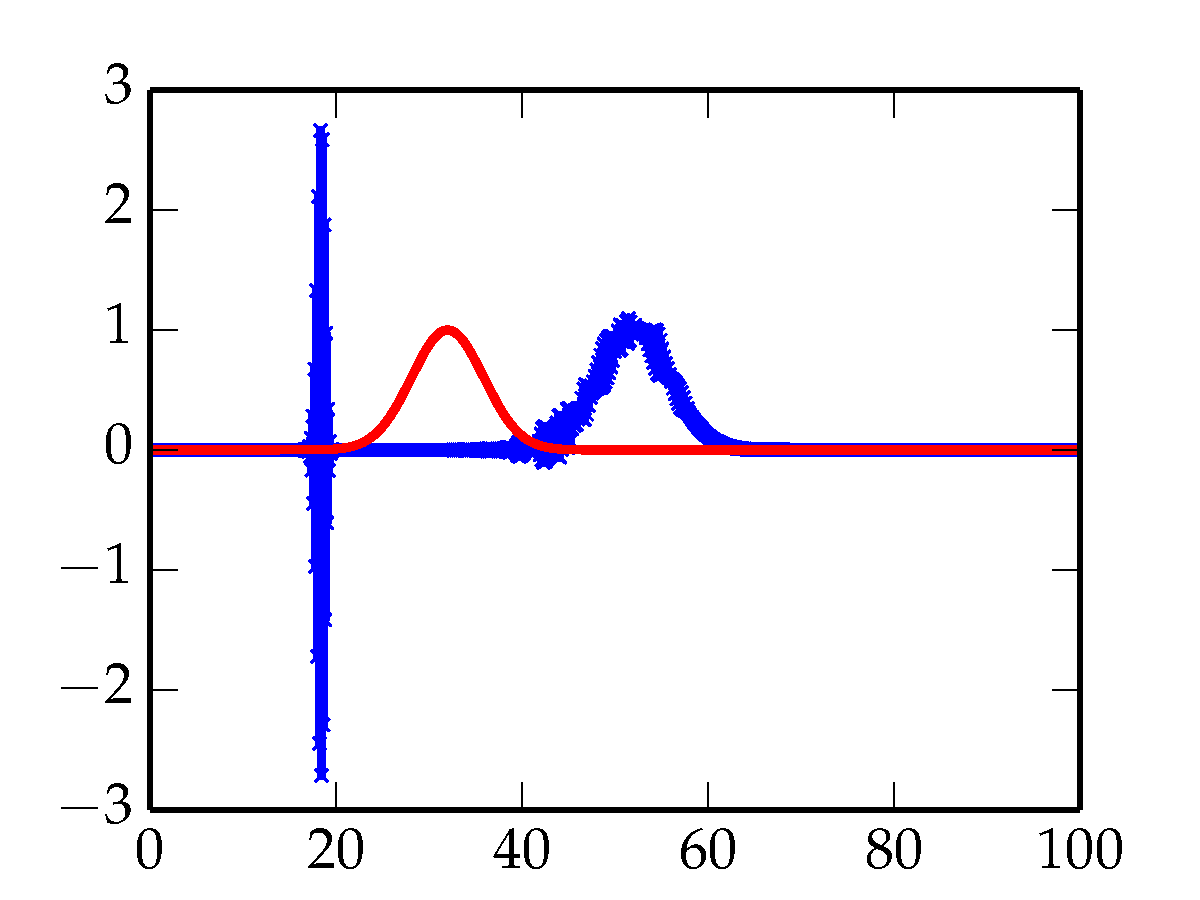
\includegraphics[width=0.5\textwidth]{fig-v-1pt1.pdf}
 \caption{The analytical (red) and upwind numerical (blue) solutions to the advection equation after 200 iterations-worth of time has passed, with \(\sigma = \sqrt{15}\) and \(v = 1.1 \Delta x / \Delta t\).}
 \label{fig-v-1pt1}
\end{figure} 

Conversely, I ran the same scheme but with \(v \Delta t / \Delta x = 0.9\), inside the range where the scheme is supposedly stable. Figure 2 depicts the solution after 400 iterations; twice as long as the computation in Figure 1 was run for before unstable behavior appeared. There is clearly no apparent instability, at least yet.	

\begin{figure}[H]
 \centering
 \hspace{0cm} 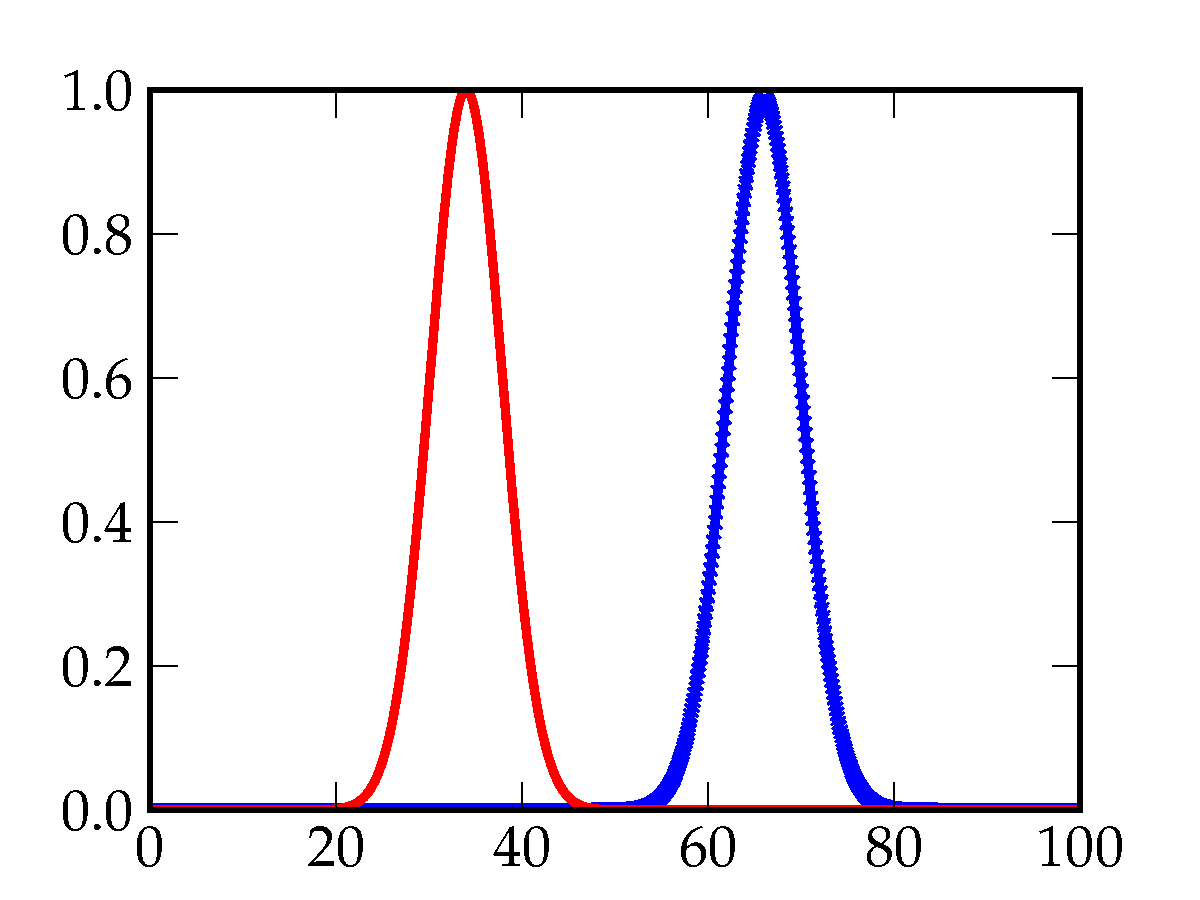
\includegraphics[width=0.5\textwidth]{fig-v-0pt9.pdf}
 \caption{The analytical (red) and upwind numerical (blue) solutions to the advection equation after 200 iterations-worth of time has passed, with \(\sigma = \sqrt{15}\) and \(v = 0.9 \Delta x / \Delta t\).}
 \label{fig-v-0pt9}
\end{figure} 

I implemented a simple error measure between the analytic result and the numerical approximation that is inspired by the Euclidean norm and the standard deviation formula; the error measure \(\varepsilon\) is
\[
\varepsilon = \sqrt{\frac{1}{N}\sum_i (y_{\text{analytic}, i} - y_{\text{numerical}, i})^2}
\]
This is proportional to the Euclidean norm of the difference between the vector \(\vec{y}_\text{analytic}\) and the vector~\(\vec{y}_\text{numerical}\). The error \(\varepsilon\) is plotted as a function of iteration number for the Gaussian with \(\sigma = \sqrt{15}\) and for the Gaussian with \(\sigma = \sqrt{15}/5\) in Figure 3.

\begin{figure}[H]
 \centering
 \hspace{0cm} 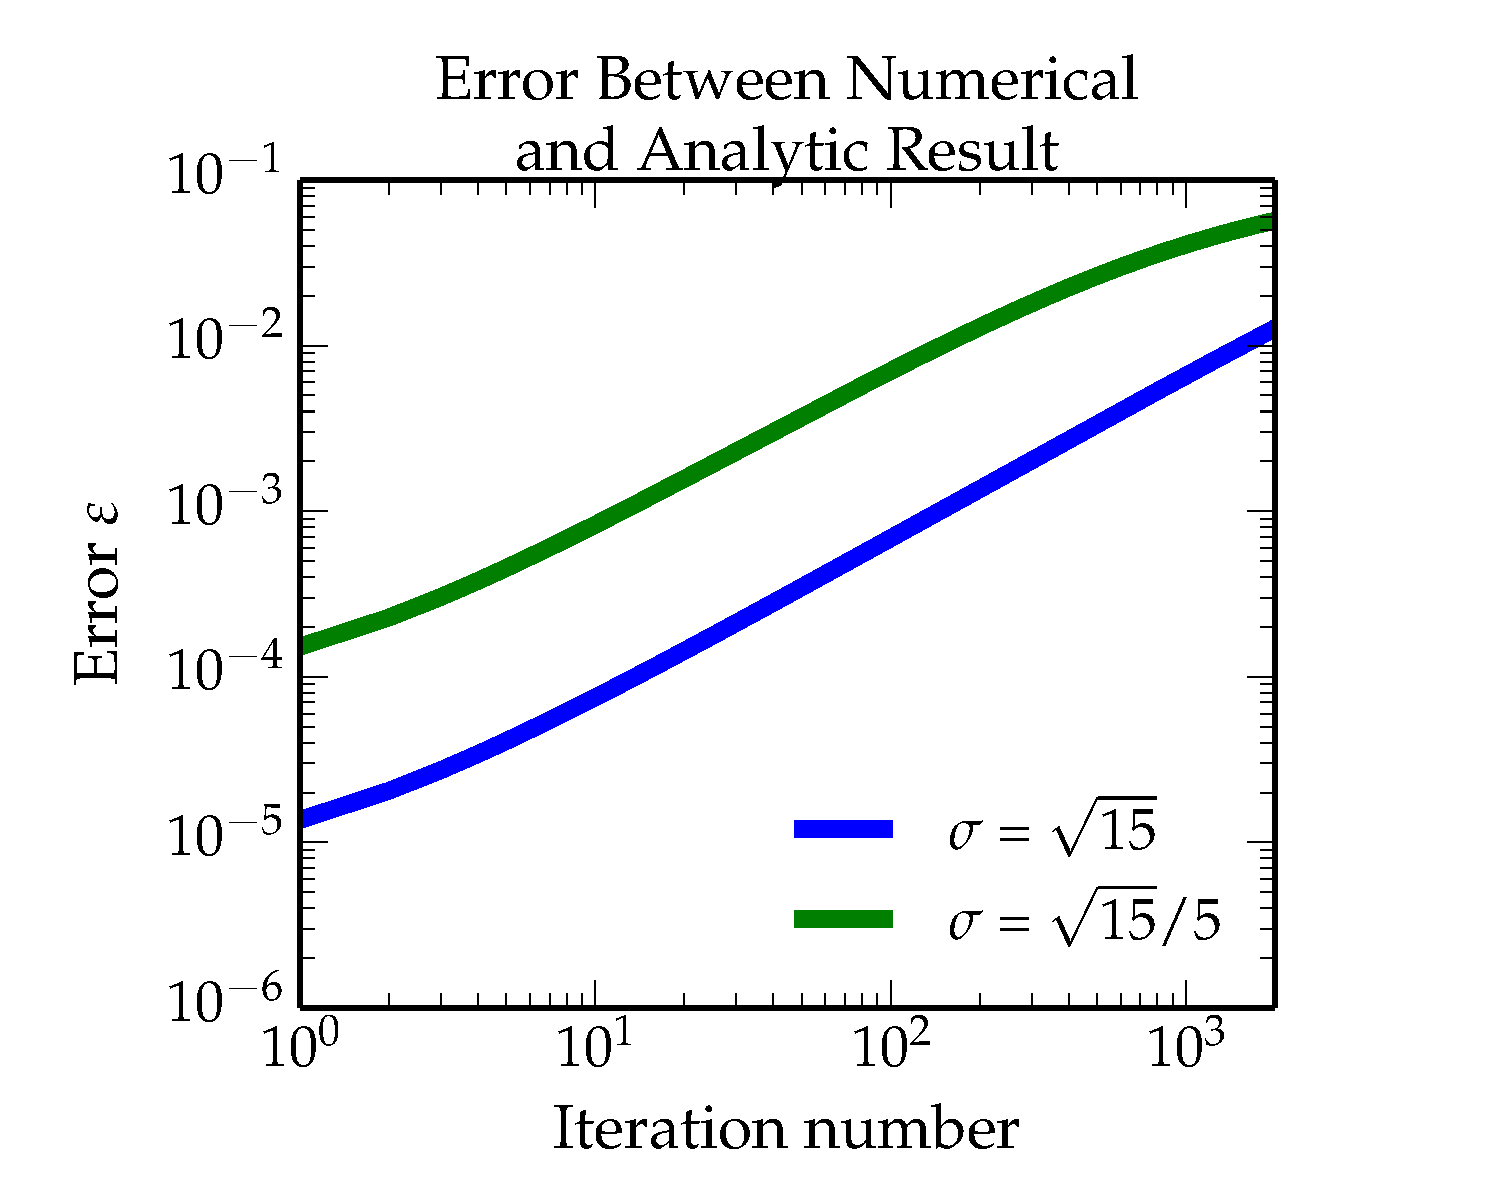
\includegraphics[width=\textwidth]{fig-errors.pdf}
 \caption{Error \(\varepsilon\) between the numerical and analytical result as a function of iteration number for two Gaussians of varying standard deviation \(\sigma\).}
 \label{fig-errors}
\end{figure} 

The Gaussian with smaller standard deviation has an order of magnitude-higher error. The narrower numerical Gaussian also decays in amplitude relative to the analytic Gaussian much faster than the wider numerical Gaussian, as demonstrated in Figures 4 and~5. Both numerical Gaussians decay, but by the time the wider Gaussian has decayed by \(\sim 5\%\), the narrower Gaussian has decayed by \(\sim 50\%\).

\begin{figure}[H]
 \centering
 \hspace{0cm} 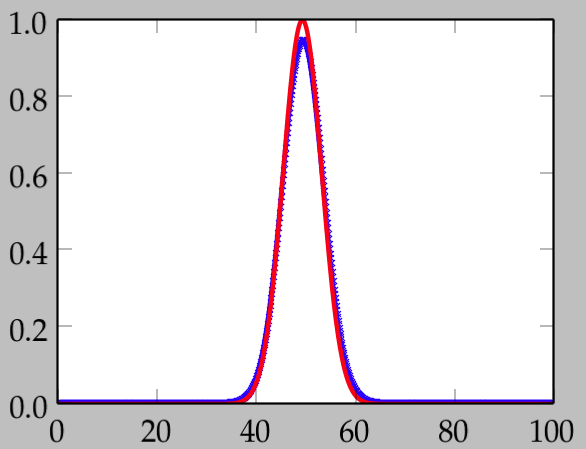
\includegraphics[width=0.5\textwidth]{fig-sigma0.png}
 \caption{The analytical (red) and upwind numerical (blue) solutions to the advection equation after 2000 iterations-worth of time has passed, with \(\sigma = \sqrt{15}\) and \(v = 0.1 \Delta x / \Delta t\).}
 \label{fig-sigma0}
\end{figure} 

\begin{figure}[H]
 \centering
 \hspace{0cm} 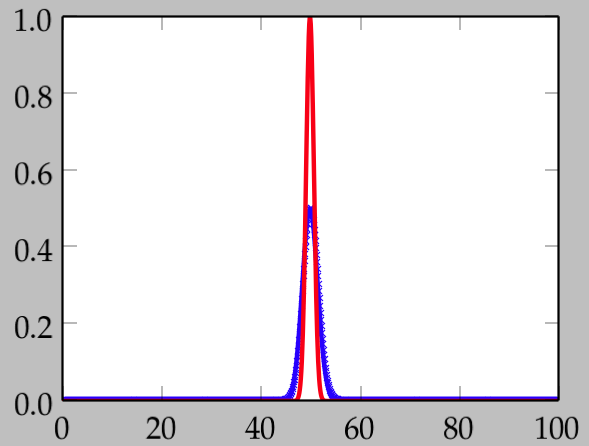
\includegraphics[width=0.5\textwidth]{fig-sigma0over5.png}
 \caption{The analytical (red) and upwind numerical (blue) solutions to the advection equation after 2000 iterations-worth of time has passed, with \(\sigma = \sqrt{15}/5\) and \(v = 0.1 \Delta x / \Delta t\).}
 \label{fig-sigma0over5}
\end{figure}

I implemented the FTCS scheme and observed the development of instability, which can be seen in Figures 6, 7, and 8.

The growing instability looks very different from the instability in the upwind scheme for \(v \Delta t / \Delta x > 1\) (Figure 1). The first difference is that the instability seems to grow fast oscillations at the left boundary in FTCS, whereas for upwind that happened at \(x\simeq20\), not the boundary. The second difference is a in FTCS a noticeable instability makes the left side of the Gaussian very noisy and distorted, whereas this is mostly absent in upwind.
\begin{figure}[H]
 \centering
 \hspace{0cm} 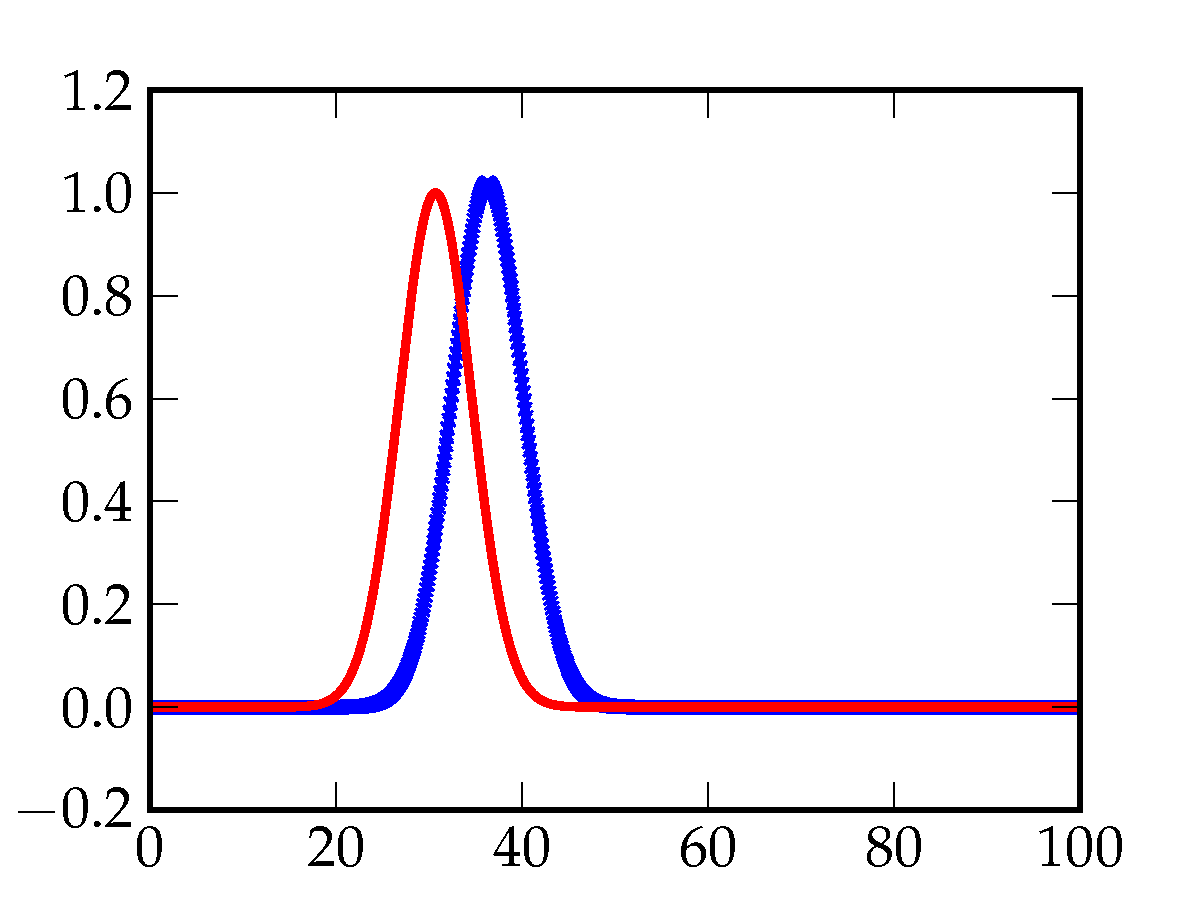
\includegraphics[width=0.4\textwidth]{fig-ftcs0.pdf}
 \caption{The analytical (red) and FTCS numerical (blue) solutions to the advection equation after 70 iterations-worth of time has passed, with \(\sigma = \sqrt{15}\) and \(v = 0.9 \Delta x / \Delta t\).}
 \label{fig-ftcs0}
\end{figure} 

\begin{figure}[H]
 \centering
 \hspace{0cm} 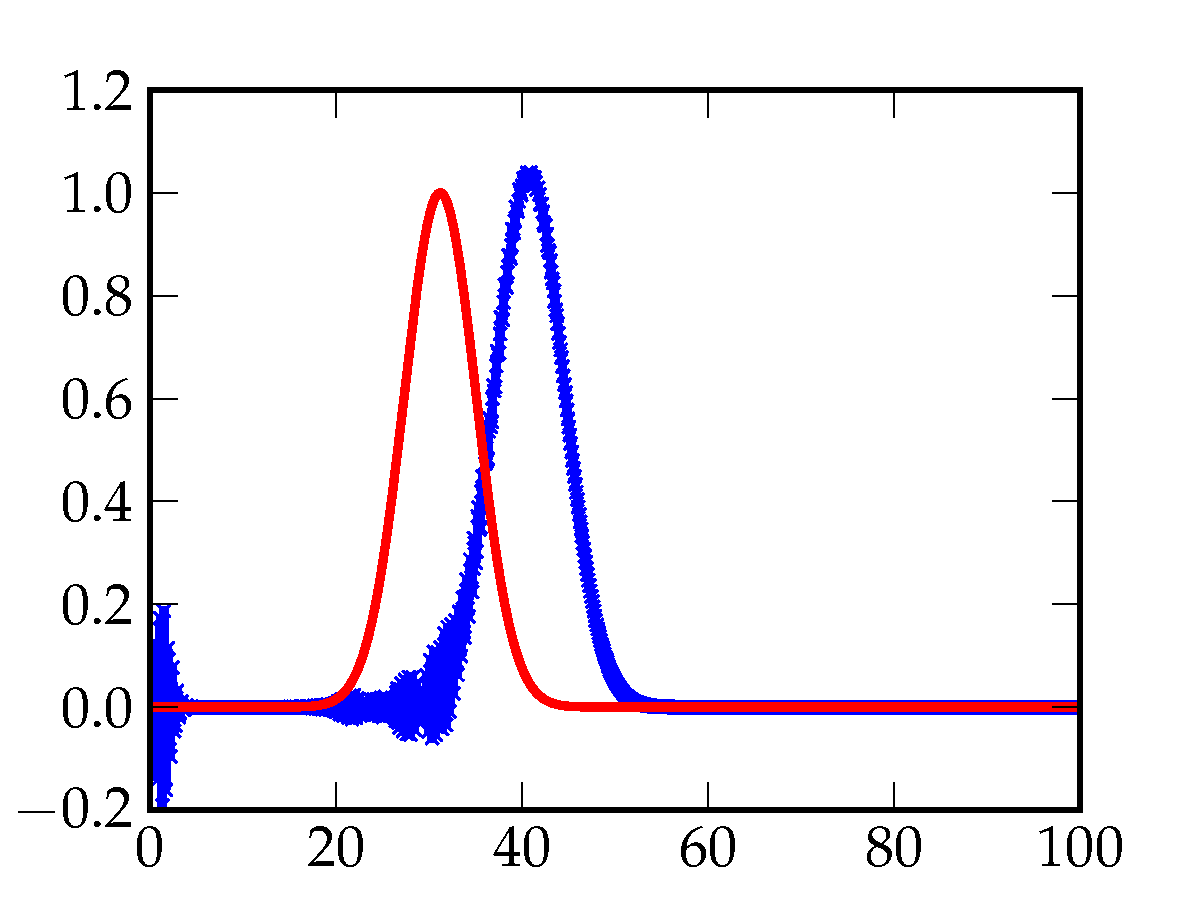
\includegraphics[width=0.4\textwidth]{fig-ftcs1.pdf}
 \caption{The analytical (red) and FTCS numerical (blue) solutions to the advection equation after 100 iterations-worth of time has passed, with \(\sigma = \sqrt{15}\) and \(v = 0.9 \Delta x / \Delta t\).}
 \label{fig-ftcs1}
\end{figure} 

\begin{figure}[H]
 \centering
 \hspace{0cm} 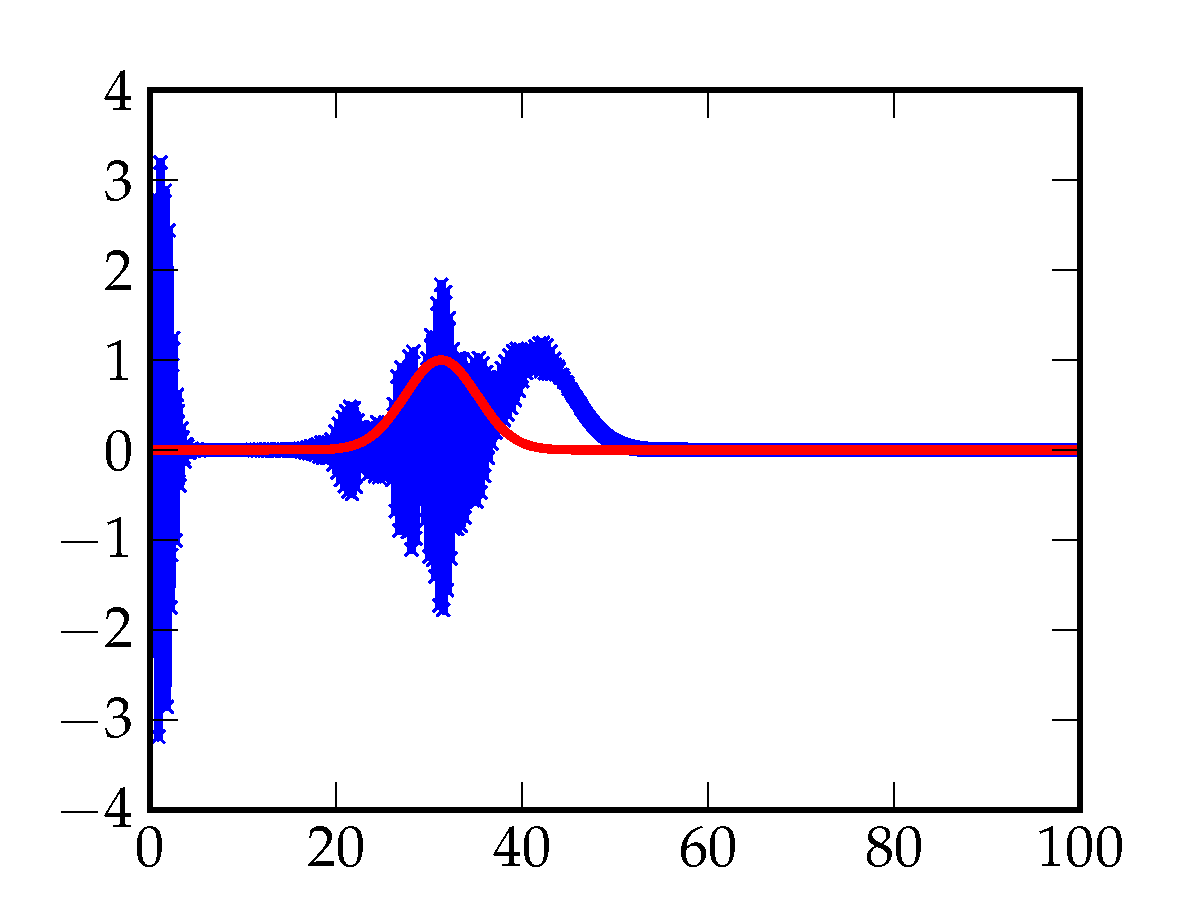
\includegraphics[width=0.4\textwidth]{fig-ftcs2.pdf}
 \caption{The analytical (red) and FTCS numerical (blue) solutions to the advection equation after 130 iterations-worth of time has passed, with \(\sigma = \sqrt{15}\) and \(v = 0.9 \Delta x / \Delta t\).}
 \label{fig-ftcs2}
\end{figure} 


\end{spacing}
\end{document}

%%%%%%%%%%%%%%%%%%%%%%%%%%%%%%%%%%%%%%%%%%%%%%%%%%%%%%%%%%%%%
